% !TeX root = thesis.tex

\chapter{Evaluation}\label{chap:evaluation}
This chapter will evaluate the performance of the previously discussed \velocity{} framework. In the first section, the projects that will be used in the experiments will be presented. The next section will formally restate the research questions that have been posed in the introduction and extend these. Afterwards, the process of how the data was obtained will be elaborated. The final section will provide answers to the research questions as well as present the results of applying \tcp{} to the test subjects.

\section{Test subjects}

\subsection{Dodona}
// Leg uit wat dodona is.


\section{Research questions}
The following research questions will be answered in the subsequent sections:

\paragraph*{RQ1: What is the probability that a test run will contain at least one failed test case?}
The first research question will provide useful insights into whether a typical test run has a tendency towards failure or success. It is expected that a typical test run will succeed.

\paragraph*{RQ2: If a run has failed, what is the probability that the next run will fail as well?}
The ROCKET algorithm (\autoref{ssec:alg-rocket}) relies on the assumption that if a test case has failed in a given run, it will most likely fail in the subsequent run as well. This research question will investigate the correctness of this hypothesis.

\paragraph*{RQ3: What is the average duration of a test run?}
Measuring how long it takes to execute a typical test run is required to estimate the benefit of applying any form of test suite optimisation.

\paragraph*{RQ4: What is the performance of applying \tcp{} to Dodona?}
This research question will investigate how quickly a failing test case in the Dodona project can be discovered using \velocity{}.

% !TeX root = ../thesis.tex

\section{Data collection}\label{sec:eval-data}

% !TeX root = ../../thesis.tex

\subsection{\travisci{} build data}
In order to answer the first three research questions, build data for several projects hosted on \travisci{} (\autoref{sssec:travisci}) was used. This data was obtained from two sources.\\

\noindent The first source is a database of $\SI{35793144}{}$ jobs, provided by Durieux et al \cite{travisanalysis}. Due to the magnitude of this dataset ($\SI{61.11}{\gibi\byte}$), a big data framework is required to parse the log files. In order to collect the required data to provide an answer to the first and third research question, two simple \texttt{MapReduce} pipelines have been executed using the Apache Spark\footnote{\url{https://spark.apache.org/}} framework..\\

\begin{figure}[htbp!]
	\centering
	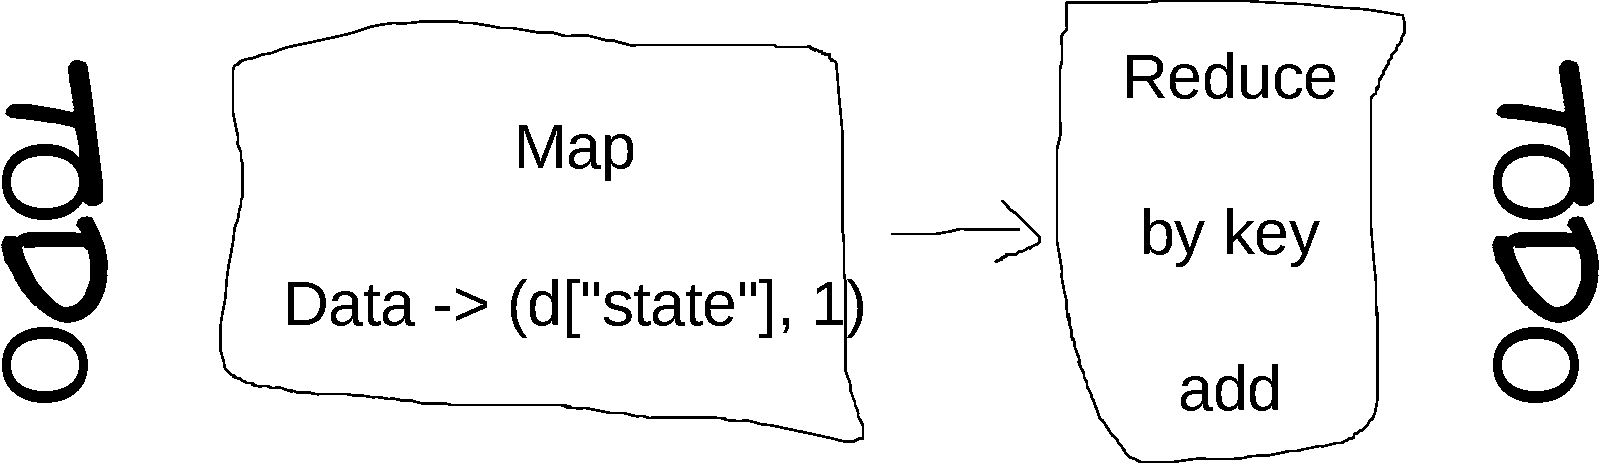
\includegraphics[width=0.8\textwidth]{assets/images/eval-rq1-mapreduce.pdf}
	\caption{MapReduce pipeline to find the failed runs}
	\label{fig:eval-mapreduce-1}
\end{figure}

\begin{figure}[htbp!]
	\centering
	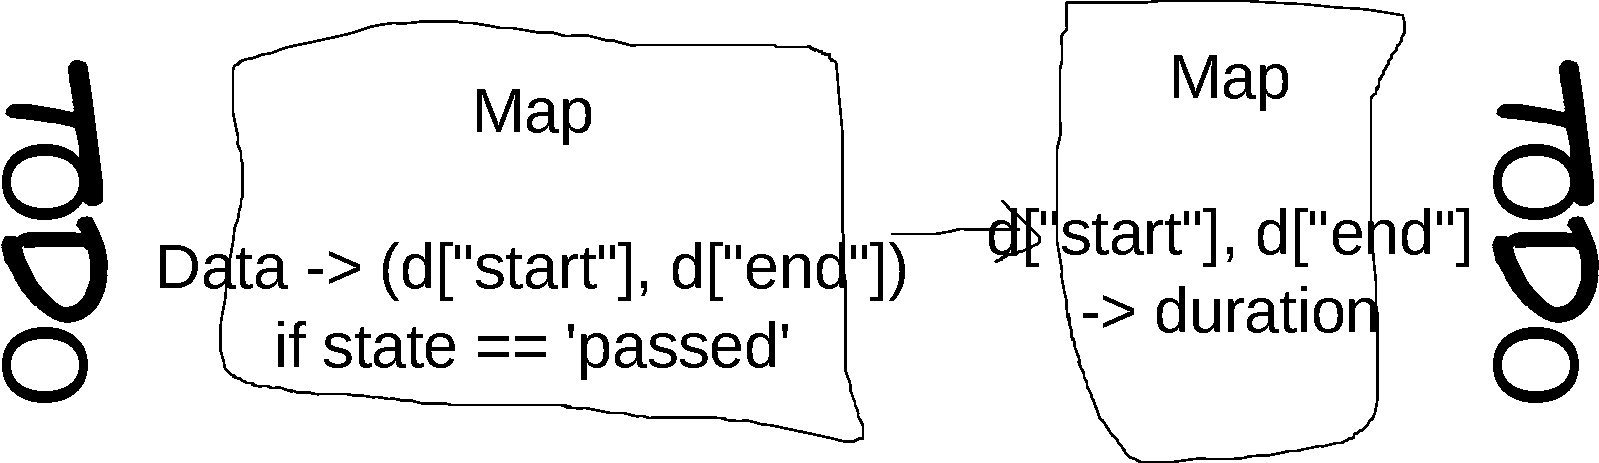
\includegraphics[width=0.8\textwidth]{assets/images/eval-rq3-mapreduce.pdf}
	\caption{MapReduce pipeline to find the average duration of a successful test run}
	\label{fig:eval-mapreduce-3}
\end{figure}

\noindent In addition to the first source, another $\SI{3702595}{}$ jobs have been analysed from the \emph{TravisTorrent} project. This project \cite{msr17challenge} scrapes the API of \travisci{} and combines this with data obtained from the \github{} API to augment the dataset with extra information. One of these additional values is the identifier of the previous executed build of every project. This identifier is required to answer the second research question. Furthermore, the amount of failed test cases in every run is included, which can be used to distinguish whether the test run has actually failed or the project could not be compiled and thus allowing a more fine-grained answer to the first research question as well. After analysis of this dataset, the execution time was not accurate compared to the actual timings on the \travisci{} build page, so this dataset was not used in the third research question. For analysis, the creators of TravisTorrent have provided a Google BigQuery\footnote{\url{https://bigquery.cloud.google.com/}} interface to allow querying the dataset, which is required given its magnitude. The following queries have been executed to obtain the required data:

\lstinputlisting[caption=TravisTorrent query: Find the amount of failed runs, label=lst:travistorrent-sql1, language=sql]{assets/listings/travistorrent-failed-runs.sql}
\lstinputlisting[caption=TravisTorrent query: Find the probability of consecutive failures,label=lst:travistorrent-sql2, language=sql]{assets/listings/travistorrent-consecutive-failures.sql}

% !TeX root = ../../thesis.tex

\subsection{Dodona data}
As mentioned before, Dodona utilises the MiniTest testing framework in conjunction with SimpleCov to calculate the coverage. MiniTest will by default only emit the name of every failed test case, without any further information. Furthermore, SimpleCov is only capable of calculating the coverage for the entire test suite and does not allow to retrieve the coverage on a per-test basis. To answer the fourth research question and apply the \velocity{} predictors to Dodona, a Python script has been created to reconstruct every failed test run. This script first queries the API of \githubactions{} to find which test runs have failed. In this thesis, $\SI{62}{}$ failed runs have been used. For every failed commit, the script retrieves the parent commit and calculates the coverage on a per-test basis. This thesis will assume that the coverage of the parent commit resembles the coverage of the failed commit. The coverage is calculated by applying the following two transformations to the parent commits and subsequently rescheduling these in \githubactions{}:

\begin{itemize}
	\item \textbf{Cobertura formatter:} The current SimpleCov reports can only be generated as HTML reports, preventing convenient analysis. This problem is resolved by using the Cobertura formatter instead, which generates XML reports. The structure of these reports is already supported by the Controller.
	
	\item \textbf{Parallel execution:} To reduce the execution time, the test cases are concurrently executed by four processes. The code coverage is recorded per process and afterwards merged. However, SimpleCov is not entirely thread-safe. This is not a problem if the total coverage is required, but it does prevent the accurate generation of per-test coverage. As a result, parallel execution has been disabled.
	
\end{itemize}

\section{Results}

1904.09416.pdf heeft een hele benchmark van 35.000.000 runs